\chapter{Konzeption und Implementation}
\section{Anforderungen}
Ziel dieser Arbeit ist es, den Xilinx Microblaze in die bestehende SpartanMC Entwicklungsumgebung zu integrieren. Um den Prozessor in JConfig einbinden zu können, müssen zunächst sowohl eine Hardwarebeschreibung, als auch eine XML-Modulbeschreibung für den Microblaze erstellt werden. Dies ist ebenso erforderlich für den UART IP-Core und den FSL-Bus IP-Core. Bei der Erstellung der Hardwarebeschreibung und der XML-Modulbeschreibung, ist darauf zu achten, dass dem Nutzer es ermöglicht wird, die Parameter der neuen Komponenten konfigurieren zu können.\\
Es ist außerdem erforderlich, dass Anpassungen an der SpartanMC Toolchain vorgenommen werden. Dies ist notwendig, um die automatische Speicherinitialisierung für den Microblaze zu ermöglichen, da die bestehende Methode der Speicherinitialisierung für den SpartanMC nicht ohne Änderungen für den Microblaze anwendbar ist. Desweiteren muss der Compiler für den Microblaze in die Toolchain integriert werden, da einige der Hardwarebeschleuniger über spezielle Instruktionen angesprochen werden. Eine Vielzahl von IP-Cores von Xilinx sind in VHDL verfasst. Da in der SpartanMC Entwicklungsumgebung IP-Cores bislang ausschließlich in Verilog verfasst wurden, ist es gegebenfalls notwendig Anpassungen an der Toolchain vorzunehmen, um VHDL Designs zu unterstützen.\\
Optional wäre es wünschenswert, die erfolgreiche Paralellisierung eines Microblaze Programms durch \textmu\/Streams zu zeigen. Hierzu wäre es notwendig, 
\textmu\/Streams soweit anzupassen, dass eine entsprechende Hardwarekonfiguration mit den neu integrierten Komponenten erstellt werden kann und
die Aufrufe der Core-Konnektoren durch Aufrufe der FSL-Blöcke ersetzt werden.
\section{Integration in JConfig}
\subsection{Hardware}
Bevor über die Integration nachgedacht werden kann, muss zunächst festgelegt werden, welche Hardware verwendet wird. Über die Jahre hat Xilinx diverse Versionen des Microblaze veröffentlicht. Die Implementationen des Prozessors sind allesamt verschlüsselt und können nur mit entsprechendem Schlüssel entschlüsselt werden. Mit der Einführung von Vivado und der Einstellung der Entwicklung von ISE änderte sich auch die Art der Verschlüsselung, sodass neuere Versionen des Microblaze nicht mehr von der alten Toolchain entschlüsselt werden können. Da die JConfig Toolchain allerdings Gebrauch von der ISE Toolchain macht, kommen für diese Arbeit nur der Microblaze v8.50c oder ältere Versionen in Frage.\\
Ausgehend vom ISE Installationsverzeichnis, ist Verzeichnis für die IP-Cores an folgender Stelle zu finden: \textit{"14.7/ISE\_DS/EDK/hw/XilinxProcessorIPLib/pcores/"}. Dort sind alle Versionen des Microblaze, sowie alle Versionen anderer Hardware abgelegt. Für sämtliche verwendete IP-Cores werden die aktuellsten Versionen verwendet.
\subsection{Hardwarebeschreibung}
\subsubsection{Erzeugung der Hardwarebeschreibung mit XPS}
Um den Microblaze in JConfig integrieren zu können, ist es zunächst notwendig, eine Hardwarebeschreibung zu erstellen, die den Microblaze instantiiert und parametrisiert.
Diese kann entweder manuell erstellt werden oder mit XPS. In XPS kann dazu mit dem Base-System-Builder ein einfaches System erzeugt werden. Ein Beispiel für ein System ohne Peripherie ist in Abbildung \ref{fig:XPS_EXAMPLE} zu sehen.
\begin{figure}[ht!]
\centering
\includegraphics[width=1\linewidth]{./bilder/XPS_EXAMPLE}
\caption{Einfaches mit XPS generiertes System ohne Peripherie}
\label{fig:XPS_EXAMPLE}
\end{figure}
Das System besteht aus einem Micorblaze, zwei LMB, zwei Speichercontroller (je einen für Daten und einen für Instruktionen), einem Block RAM als Programm- und Datenspeicher, einem AXI4-Light-Bus zur Anbindung von Peripherie, einem Reset-Core, einem Taktgenerator und einem Debug Modul. Um die Komplexität des Systems und somit zusätzliche Fehlerquellen zu reduzieren, werden der AXI4-Light-Bus, der Taktgenerator und das Debug Modul zunächst entfernt. Der AXI4-Bus wird nicht benötigt, da es zunächst in der SpartanMC Entwicklungsumgebung mit dem UART IP-Core nur eine Peripherie geben wird und diese direkt mit dem Prozessor verbunden werden kann. Der Taktgenerator wird nicht benötigt, da JConfig bereits über eigene Taktgeneratoren verfügt und das Debug Modul wird nicht benötigt, um die grundsätzliche Lauffähigkeit eines Microblaze Systems zu gewährleisten, sondern nur um Softwareanwendungen zu debuggen.\\
Nun kann in XPS eine Netzliste erzeugt werden. Als Nebenprodukt werden Wrapperdateien erstellt, die die einzelnen Komponenten mit den, im XPS angegebenen Einstellungen instantiieren. Die erzeugten Dateien werden nach Möglichkeit in der präferierten Sprache erzeugt, allerdings funktioniert dies bei manchen Wrapper Dateien nicht und sie werden in VHDL generiert. Die Top-Level-Beschreibung, welche sämtliche Komponenten instanziiert und miteinander verbindet, kann allerdings auch in Verilog erzeugt werden. Desweiteren besitzt die Top-Level-Beschreibung lediglich die, im XPS als extern makierten Signale als Eingänge und Ausgänge. Die Wrapper Datei für das Block RAM stellt eine Besonderheit dar. Für das Block RAM wird nämlich, entsprechend der angegebenen Größe des Speichers, ein elaboriertes Modell erzeugt. Dieses Modell funktioniert nur für die angegebene Speichergröße und lässt sich ohne großen Aufwand auch nicht ändern. Als Lösung des Problems wird ein generisches Speichermodul in Verilog geschrieben, welches das Verhalten der elaborierten Blöcke nachahmt (siehe \ref{subsubsec:genMem}).\\
Um nun eine konfigurierbare Hardwarebeschreibung zu erhalten, ist es notwendig, den Wrapper Dateien und der Top-Level-Beschreibung Parameter hinzuzufügen. So können bei der Instanziierung des Top-Level-Moduls Parameter übergeben werden, die dann wiederum bei der Instanziierung der einzelnen Komponenten des Systems an diese weitergegeben werden können. Ebenso ist es erforderlich, dass Signale die verwendet werden sollen, als Eingänge bzw. Ausgänge der Top-Level-Beschreibung hinzugefügt und über Signale mit der entsprechenden Komponente verbunden werden. Für den Microblaze sind dies, neben Takt- und Reset-Signalen, Signale für den Programm- und Datenspeicher, AXI4-Signale und Signale, die dem FSL-Interface zuzuschreiben sind.\\
Unter Berücksichtigung der XML-Modulbeschreibung, ist es notwendig, den Speicher als externes Modul zu handhaben, da die XML-Syntax für Prozessoren keine integrierten Speicher unterstützt. Hierzu werden die Speichercontroller und das Block RAM in einem weiterem Modul zusammengefasst (siehe \ref{subsubsec:genMem}), sodass das Modul für den Microblaze noch aus den Instanzen für den Microblaze, den beiden LMB und dem Reset-Core besteht. Die LMB-Cores erlauben es mehr als einen Speicher an den Microblaze anzuschließen.\\
Welche Parameter für die Konfiguration des Microblaze wichtig sind, wird im nächsten Abschnitt behandelt. 
\subsubsection{Handhabung der Parameter}
In diesem Kapitel wird behandelt, welche Parameter für die Konfiguration des Microblaze-Systems wichtig sind.
Für die Parameter des Microblaze wurde die Tabelle aus dem Abschnitt \textit{MicroBlaze Core Configurability} in Kapitel 3 des Microblaze Datenblattes <Referenz einfügen> herangezogen. Parameter, die in der Tabelle nur einen Wert in der Spalte \textit{Allowable Values} haben, werden fest auf diesen Wert gesetzt und können nicht vom Anwender verändert werden. In der Tabelle \ref{tab:MicParam} werden lediglich die Parameter behandelt, welche mehr als einen erlaubten Wert haben, allerdings trotzdem auf einen festen Wert gesetzt werden. Alle anderen Parameter, die nicht genannt werden, stehen dem Nutzer zur freien Konfiguration zur Verfügung. Erklärungen zu den Bedeutungen der einzelnen Parametern werden in Kurzform in der XML-Modulbeschreibung hinterlegt, sodass der Nutzer während der Erstellung eines Systems weiß, welche Funktion die einzelnen Parameter haben. Für detailliert Beschreibungen sei noch einmal auf das Datenblatt des Microblaze verwiesen. %TODO EInfügen einer Referenz
\begin{table}[ht!]
	\begin{tabular}{|l|c|p{10cm}|}
		\hline \textbf{Parameter} & \textbf{Wert} & \textbf{Beschreibung} \\ 
		\hline C\_LOCKSTEP\_SLAVE & 0 & Im Lockstep Modus können zwei oder mehrere \newline Microblaze das selbe Programm ausführen und die Ergebnisse miteinander vergleichen, um Hardwarefehler zu erkennen. Wird nicht benötigt.\\ 
		\hline C\_ENDIANNESS & 1 & Endianness wird auf Little Endian festgelegt. In XPS lässt sich dieser Wert nicht manuell verändern, dementsprechend wird auch unter JConfig darauf verzichtet.\\ 
		\hline C\_D\_AXI & 1 & Das AXI-Daten-Interface kann verwendet werden. \\ 
		\hline C\_I\_AXI & 1 & Das AXI-Instruktionen-Interface kann verwendet werden. (Nützlich bei externen Speicher) \\ 
		\hline C\_D\_PLB & 0 & Da bereits AXI verwendet wird, wird der PLB Bus nicht gebraucht und deshalb deaktiviert. \\ 
		\hline C\_I\_PLB & 0 & Siehe vorheriger Eintrag. \\ 
		\hline C\_D\_LMB & 1 & Das LMB-Daten-Interface kann verwendet werden. \\ 
		\hline C\_I\_LMB & 1 & Das LMB-Instruktionen-Interface kann verwendet werden. \\ 
		\hline C\_IPLB\_BUS\_EXCEPTION & 0 & Da der PLB nicht verwendet wird, werden die Exceptions auch nicht benötigt. \\ 
		\hline C\_DPLB\_BUS\_EXCEPTION & 0 & Siehe vorheriger Eintrag. \\ 
		\hline C\_ADDR\_TAG\_BITS & 17 & Das Datenblatt gibt kaum nützliche Informationen zu diesem Parameter, daher wird er auf den Default-Wert festgesetzt. \\ 
		\hline C\_DCACHE\_ADDR\_TAG & 17 & Siehe vorheriger Eintrag. \\ 
		\hline C\_USE\_EXT\_BRK & 0 & Siehe vorheriger Eintrag. \\ 
		\hline C\_USE\_EXT\_NM\_BRK & 0 & Siehe vorheriger Eintrag. \\ 
		\hline 
	\end{tabular}
	\centering
	\caption{Parameter des Microblaze die mehr als einen erlaubten Wert haben, aber dennoch auf einen Wert festegelegt werden.}
	\label{tab:MicParam}
\end{table}
Neben dem Microblaze werden mit einem generischen Speichermodul, einem UART-Modul und einem FSL-Modul noch drei weitere Module für JConfig erstellt, die parametrisiert werden können. Welche Parameter zur Verfügung stehen und was diese bewirken ist in den nachstehenden Tabellen aufgeführt.

\begin{table}[ht!]
	\begin{tabular}{|l|p{10cm}|}
		\hline \textbf{Parameter} & \textbf{Beschreibung} \\ 
		\hline C\_FAMILY & Dieser Parameter wird von Xilinx IP-Cores verwendet, um, je nach verwendeter Hardware, vorhandene Primitives zu instantiieren. \\ 
		\hline RAMBLOCKS & Ähnlich wie für den Speicher des SpartanMC, kann angegeben werden, wie viel RAM instantiiert werden soll. Ein Block ist jeweils 2KB groß. Es können nur Größen gewählt werden, die einer Potenz von Zwei entsprechen, da mit jeder Vergrößerung des Speichers sich die Anzahl der Bitlanes verdoppelt.\\ 
		\hline C\_BASEADDRESS & Gibt die Startaddresse des Speichers an.\\ 
		\hline 
	\end{tabular}
	\centering
	\caption{Parameter des Speichermoduls für den Microblaze.}
	\label{tab:MemParam}
\end{table}

\begin{table}[ht!]
	\begin{tabular}{|l|p{10cm}|}
		\hline \textbf{Parameter} & \textbf{Beschreibung} \\ 
		\hline C\_S\_AXI\_ACLK\_FREQ\_HZ & Frequenz des Taktsignals, welches automatisch aus dem Takt abgeleitet wird.\\ 
		\hline C\_FAMILY & Dieser Parameter wird von Xilinx IP-Cores verwendet, um, je nach verwendeter Hardware, vorhandene Primitives zu instantiieren.\\ 
		\hline C\_BAUDRATE & Für die Übertragung verwendete Baudrate. Werte von 110 bis 921600 sind möglich \\ 
		\hline C\_DATABITS & Anzahl der zu übertragenden Bits pro Frame. Werte von 5 bis 8 sind möglich. \\ 
		\hline C\_USE\_PARITY & Gibt an, ob ein Paritätsbit mit übertragen wird. \\ 
		\hline C\_ODD\_PARITY & Gibt an, ob die Parität gerade oder ungerade ist. \\ 
		\hline 
	\end{tabular}
	\centering
	\caption{Parameter des UART-Cores.}
	\label{tab:UARTParam}
\end{table}

\begin{table}[ht!]
	\begin{tabular}{|l|p{10cm}|}
		\hline \textbf{Parameter} & \textbf{Beschreibung} \\ 
		\hline C\_EXT\_RESET\_HIGH & Gibt an ob das externe Reset-Signal high-aktiv oder low-aktiv ist.\\ 
		\hline C\_ASYNC\_CLKS & Gibt an, ob das FSL-Interface synchron oder asyncron betrieben werden soll.\\ 
		\hline C\_IMPL\_STYLE & Wenn dieser Parameter auf 0 gesetzt ist, wird der FIFO-Speicher mit LUT RAMs implementiert, andernfalls mit Block RAMs.   \\ 
		\hline C\_USE\_CONTROLL & Bestimmt, ob das Steuerbit mit übertragen wird oder nicht.\\ 
		\hline C\_FSL\_DWIDTH & Ist auf 32 Bit festgelegt, da andere Datenbreiten im Zusammenhang mit dem Microblaze wenig sinnvoll sind. \\ 
		\hline C\_FSL\_DEPTH & Beschreibt die Größe des FIFO-Speichers. Diese ist von den Parametern C\_ASYNC\_CLKS und C\_IMPL\_STYLE abhängig. C\_ASYNC\_CLKS=0 => 1-8192. C\_ASNYNC\_CLKS=1 und C\_IMPL\_STYLE=0 => 16-128. C\_ASNYNC\_CLKS=1 und C\_IMPL\_STYLE=1 => 512-8192. Ist C\_ASNYNC\_CLKS=1 muss die Größe außerdem einer Potenz von Zwei entsprechen.\\ 
		\hline C\_READ\_CLOCK\_PERIOD & Wird automatisch aus dem Taktsignal berechnet. Wird genutzt um Timing Constraints für den asynchronen Pfad durch LUT RAMs zu erzuegen \\
		\hline 
	\end{tabular}
	\centering
	\caption{Parameter des FSL-Cores.}
	\label{tab:FSLParam}
\end{table}

\subsubsection{Implementation eines generischen Speichermoduls} \label{subsubsec:genMem}
Bevor über eine Implementation eines generischen Speichermoduls nachgedacht werden kann, sollte zunächst die Struktur, des von Xilinx verwendeten Speichers erläutert werden. Hierzu wird Abbildung \ref{fig:XilinxMEM} herangezogen.
\begin{figure}[ht!]
\centering
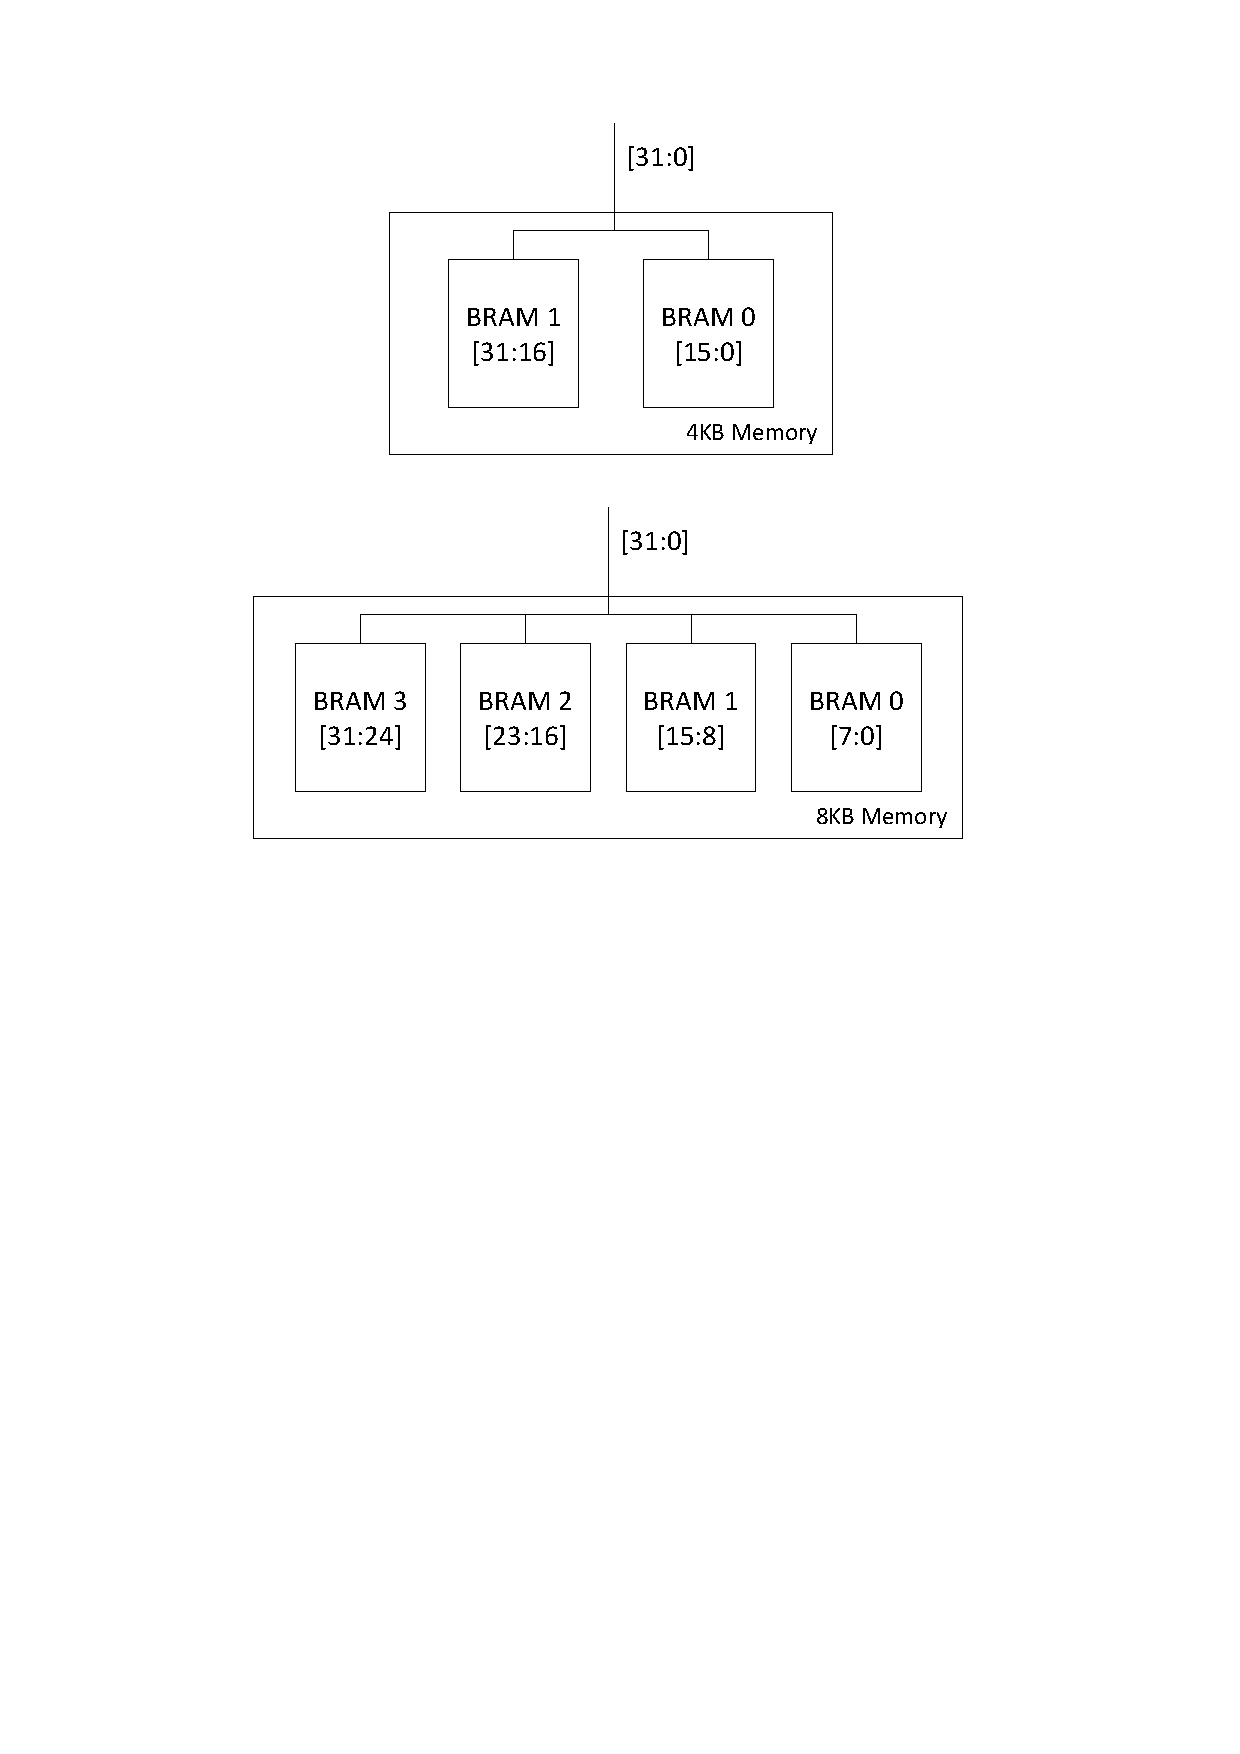
\includegraphics[width=0.7\linewidth]{./bilder/XilinxMEM}
\caption{Speicherstruktur der von Xilinx generierten Speichermodule}
\label{fig:XilinxMEM}
\end{figure}
In der Abbildung sind einfache Blockschaltbilder für einen 4KByte und einen 8KByte großen Speicher dargestellt. Angefangen bei einer Mindestgröße von 2KByte verdoppelt sich die Anzahl der Block RAMs bei jeder Vergrößerung. Dabei halbiert sich jeweils die Größe der Bitlanes bis hin zu einem Minimum von eins bei einer maximalen Speichergröße von 64KByte. Die vom XPS generierten Modelle instantiieren immer eine fixe Anzahl an Block RAMs, sodass es nicht möglich ist, mit der selben Methode wie beim Microblaze eine generische Parametriserbarkeit herzustellen. Daher muss, auf Grundlage der elaborierten Modelle, ein generisches Speichermodul geschrieben werden, dessen Größe über einen Parameter festgelegt werden kann.\\
Um dies zu erreichen, wird ein Verilog-Modul geschreiben, welches die Parameter \textit{RAMBLOCKS} und \textit{C\_FAMILY} hat. Über eine for-Schleife in einer generate-Umgebung werden entsprechend des Parameters \textit{RAMBLOCKS} Block RAMS instantiiert. Eine Funktion berechnet dabei aus dem Parameter die Breite der einzelenen Bitlanes. Um die Signalverbidungen zu realisieren, werden wires und regs deklariert, deren Größe mit \textit{RAMBLOCKS} skaliert. Über Indexing wird innerhalb der for-Schleife die Realisierung der einzelnen Bitlanes vorgenommen. Für das 4-Bit breite Write-Enable-Signal wird zusätzliche Kombinatorik hinzugefügt, da die Handhabung nicht durch einfaches Indexing umgesetzt werden kann.

\subsection{Modulbeschreibungen}

\subsection{Busbeschreibungen}

\subsection{Änderungen an JConfig}

\section{Integration in die SpartanMC Toolchain}
\subsection{Ausgangslage}

\subsection{Zusätzlich benötigte Informationen}

\subsection{Weitere Änderungen an JConfig}

\subsection{Änderungen an der Toolchain}

